\chapter{Results}\label{chapter:results}

The \texttt{AlgorithmAnalysis.jl} package's ability to perform automatic algorithm analysis have been tested on GD, FG, HB. We have also tested on Triple-momentum (TMM), which was proven to be the fastest known globally convergent algorithm for minimizing smooth strongly convex functions in \cite{TMM}. In \cite{tutorial}, these four algorithms were tested with $m$-strong $L$-smooth convex function class over a range of $m/L$ condition numbers between one and 100. To show the package's ability to accurately analyze algorithms for worst-case performance guarantees, we seek to replicate the analysis results presented in Fig.~2 of \cite{tutorial} with results derived from running \texttt{AlgorithmAnalysis.jl} over the same range of condition numbers. The analysis results are presented in \cref{4_results}.

\begin{figure}[h]
    \centering
    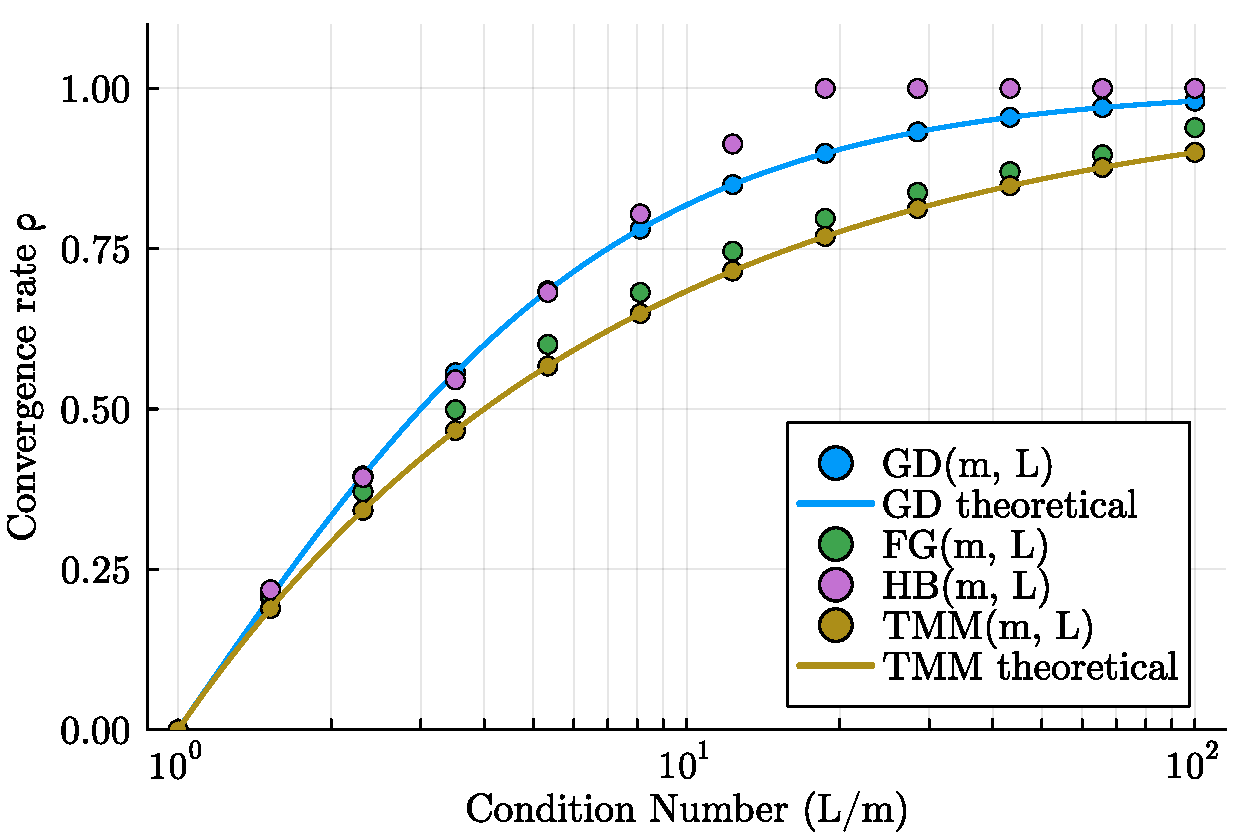
\includegraphics[width = .8 \textwidth]{results.pdf}
    \caption{Convergence rate guarantee of four algorithms over smooth strongly convex function class}
    \label{4_results}
\end{figure}

To create \cref{4_results}, we set the value of $m$ to 1 and sample 12 values of $L$ that are logarithmically spaced between 1 and 100, using a base-10 scale. The convergence rate produced by the package is plotted on the y-axis, while the x-axis plots the condition number $L/m$ of the tested $(m,L)$ values. Also included in \cref{4_results} is the theoretical performance limit of the TMM algorithm at optimizing smooth strongly convex function presented in \cite{TMM}. Every algorithm analyzed were lifted using a lifting dimension of one.

Comparing \cref{4_results} with Fig. 2 of \cite{tutorial} and Fig. 1 of \cite{TMM}, we find the analysis result produced by \texttt{AlgorithmAnalysis.jl} matches that in \cite{tutorial} for all four algorithms GD, FG, HB, and TMM. This proves the package's ability to accurately analyze these algorithms for smooth strongly convex functions.

\subsection*{Gradient descent}

To analyze GD, we use stepsize $\alpha = 2/(L+m)$ similar to \cref{ex_analysis} and that used in \cite{tutorial}. The code used to generate GD(m, L) in \cref{4_results} is presented in \cref{gd_code} with \texttt{m} set to one, \texttt{L} set to the sampled $L$ values, and \texttt{lifting\_dimension} set to one.

\begin{figure}[h!]
	\begin{lstlisting}[mathescape]
$\alpha$ = 2/(L+m)
@algorithm begin    
    f = DifferentiableFunctional{R$^n$}()
    f $\in$ SmoothStronglyConvex(m, L)
    xs = first_order_stationary_point(f)
    x0 = R$^n$()
    x1 = x0 - $\alpha$*f'(x0)
    x0 => x1
    lift(x1, lifting_dimension)
    performance = (x0-xs)^2
end
@show rate(performance, prev_rate)
\end{lstlisting}
\caption{Analysis of gradient descent and $m$-$L$ sector bounded functions}
\label{gd_code}
\end{figure}

We have also tested the same gradient descent algorithm over a function class where the gradient is $(m, L)$ sector-bounded. The code used to find the worst-case convergence rate guarantees of the fast gradient algorithm at optimizing $(m, L)$ sector-bounded function classes is identical to the code used for GD on smooth strongly convex function, but with command
\begin{lstlisting}[mathescape]
    f' $\in$ SectorBounded(m, L, xs, f'(xs))
\end{lstlisting}
replacing the command \texttt{f $\in$ SmoothStronglyConvex(m, L)}. The plot of the result produced is presented in Figure \ref*{gd_sectorbounded_results}.

\begin{figure}[h]
    \centering
    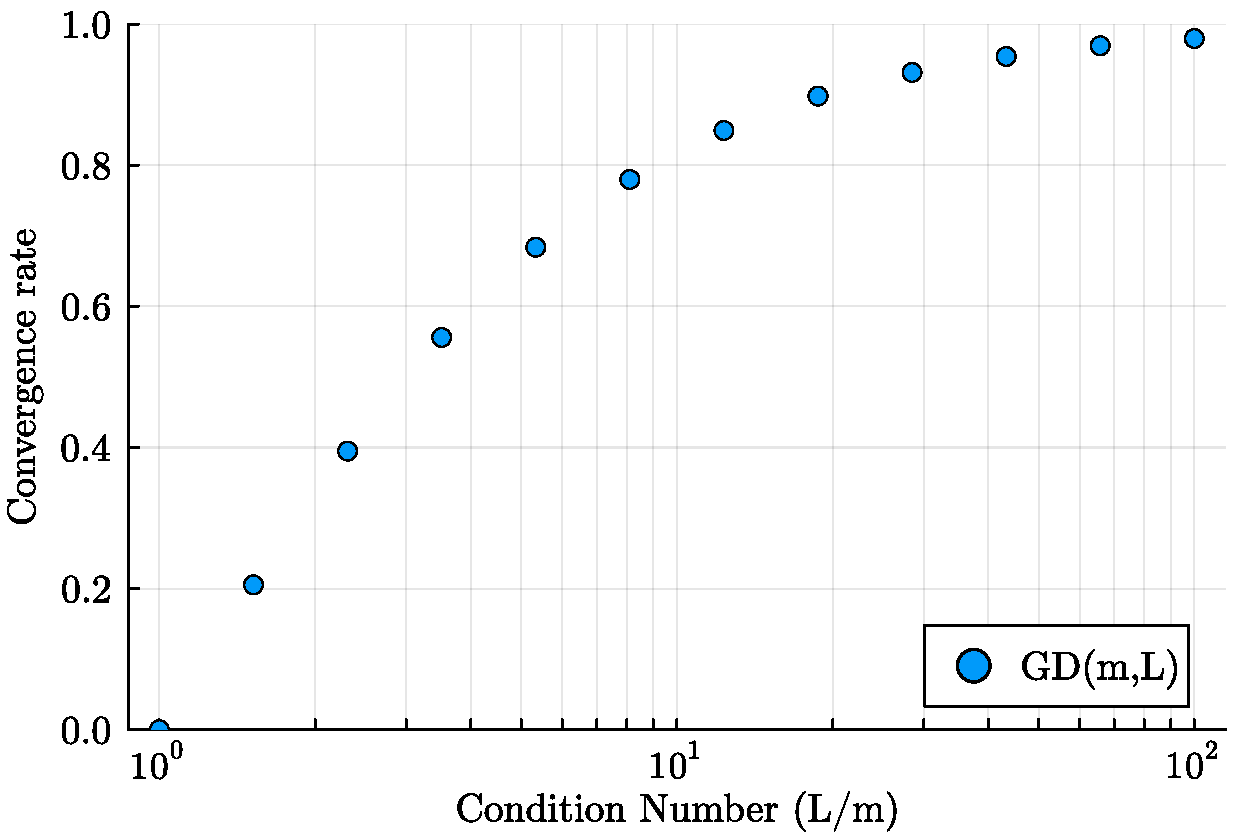
\includegraphics[width = .8 \textwidth]{gd_sectorbounded_results.pdf}
    \caption{Convergence rate guarantee of gradient descent over sector bounded function class}
    \label{gd_sectorbounded_results}
\end{figure}

In order to measure the effect of creating additional state iterates on the convergence rate guarantee found, we plot the results of analyzing GD with the same parameters as those used to create \cref{4_results} but with \texttt{lifting\_dimension} values zero and one. The analysis result is presented in \cref{GDresults}, from which we can see that additional lifting does not affect the performance guarantee found for GD.

\begin{figure}[h]
    \centering
    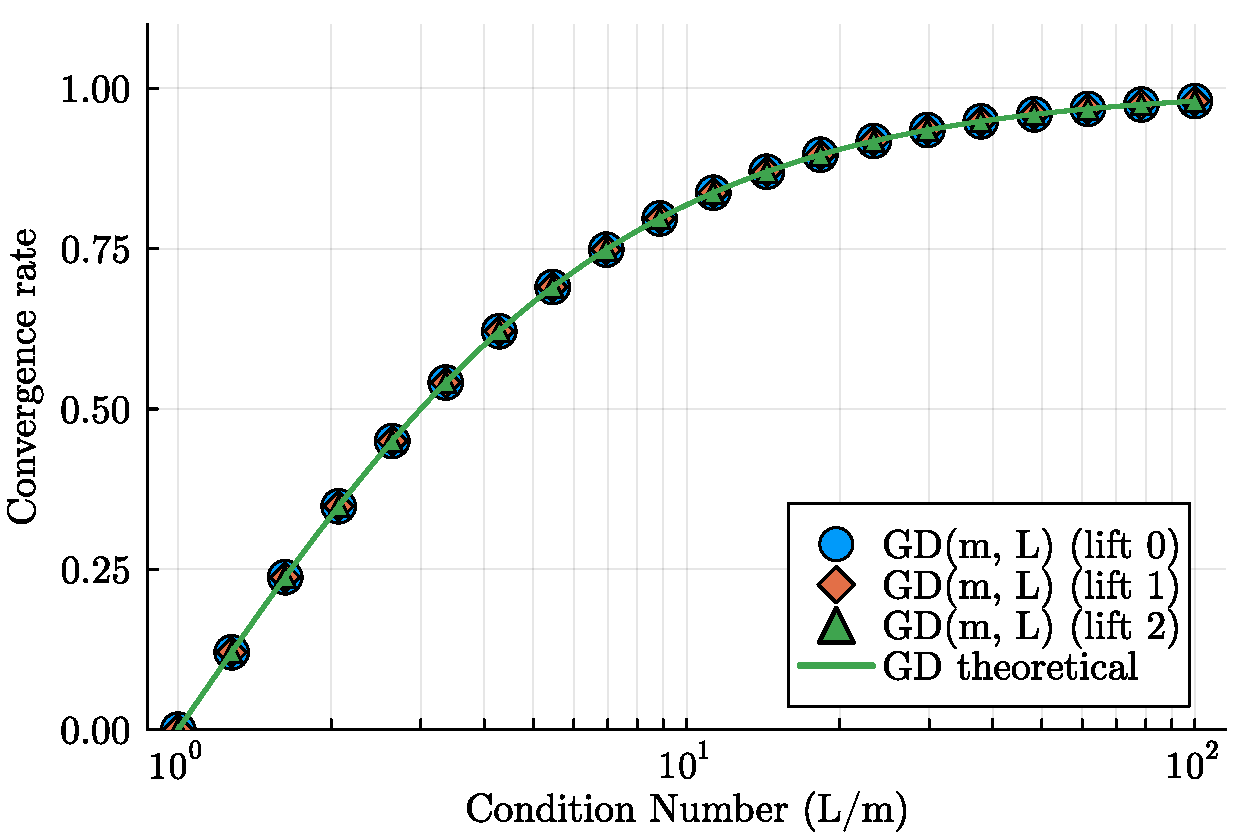
\includegraphics[width = .8 \textwidth]{GDresults.pdf}
    \caption{Convergence rate guarantee of gradient descent lifting dimensions zero and one, over smooth strongly convex function class}
    \label{GDresults}
\end{figure}

\subsection*{Fast gradient}

We tested the fast gradient algorithm with step sizes similar to that used in \cite{tutorial}:
\[
\alpha = \frac{4}{3L + m}, \quad
\beta = \frac{\sqrt{3L + 1} - 2}{\sqrt{3L + 1} + 2}
\]

The code used to find the worst-case convergence rate guarantees of the FG algorithm in \cref{4_results} is presented in \cref{fg_code}, with \texttt{m} set to one, \texttt{L} set to the sampled $L$ values, and \texttt{lifting\_dimension} set to one.

\begin{figure}[h!]
	\begin{lstlisting}[mathescape]
$\alpha$ = 4/(3*L+m); $\beta$=(sqrt(3*L+1)-2)/(sqrt(3*L+1)+2)
@algorithm begin
    f = DifferentiableFunctional{R$^n$}()
    xs = first_order_stationary_point(f)
    f $\in$ SmoothStronglyConvex(m, L)
    x0 = R$^n$()
    x1 = R$^n$()
    y1 = x1 + $\beta$*(x1 - x0)
    x2 = y1 - $\alpha$*f'(y1)
    x0 => x1
    x1 => x2
    lift(x2, lifting_dimension)
    performance = (y1-xs)^2
end
@show rate(performance)
\end{lstlisting}
\caption{Analysis of fast gradient and $L$-smooth $m$-strongly convex functions}
\label{fg_code}
\end{figure}

In order to see the effect of lifting on the convergence rate guarantee found, we plot the results of analyzing FG with \texttt{lifting\_dimension} values of zero, one, and two. The analysis result is presented in \cref{FGresults}. We can see that while there is no difference in the analysis result between a creating one or two more iterates than the minimum, a lifting dimension of zero gives the incorrect result compared to Fig.2 of \cite{tutorial}.

\begin{figure}[h]
    \centering
    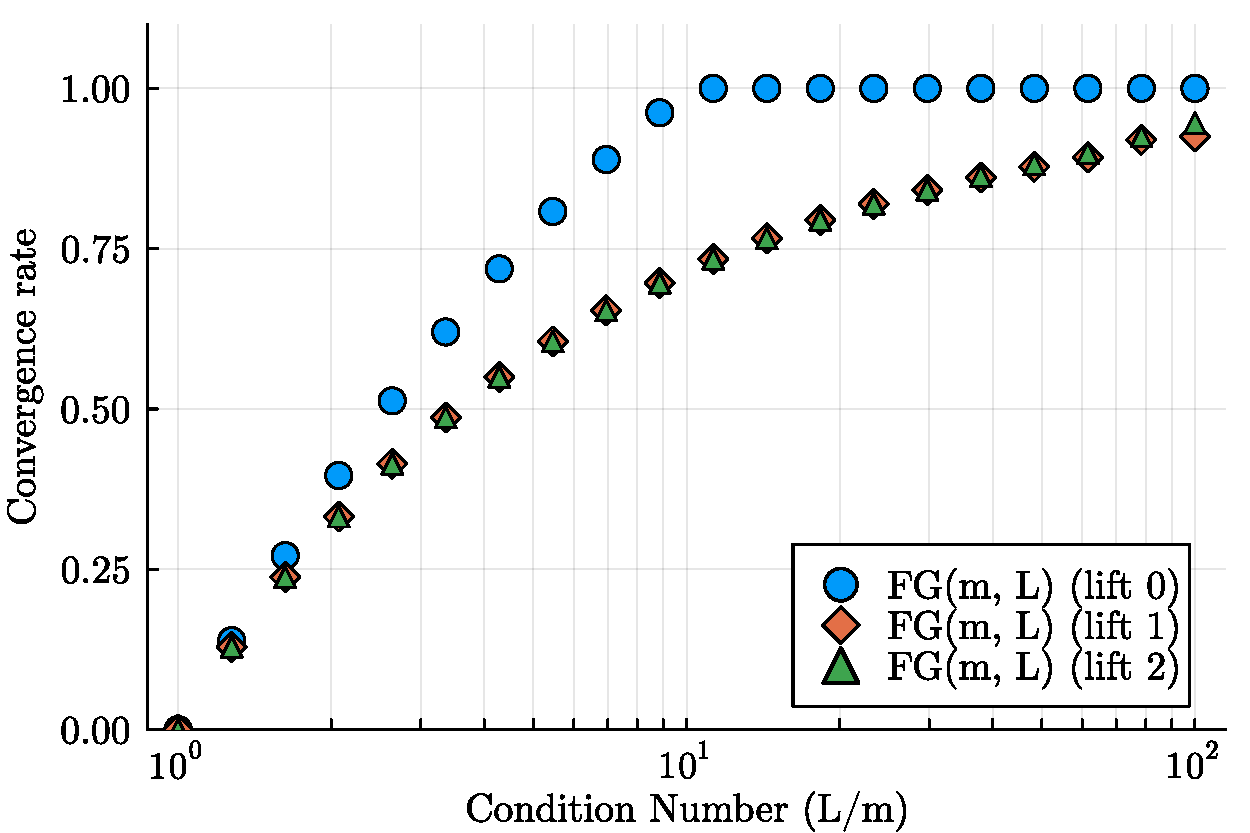
\includegraphics[width = .8 \textwidth]{FGresults.pdf}
    \caption{Convergence rate guarantee of fast gradient with lifting dimensions zero, one, and two, over smooth strongly convex function class}
    \label{FGresults}
\end{figure}

\subsection*{Heavy ball}

We tested the heavy ball algorithm with step sizes similar to that used in \cite{tutorial}:
\[
\alpha = \frac{4}{\left( \sqrt{L} + \sqrt{m} \right)^2}, \quad
\beta = \left( \frac{\sqrt{L/m} - 1}{\sqrt{L/m} + 1} \right)^2
\]

The code used to find the worst-case convergence rate guarantees of the heavy ball algorithm for optimizing $m$-strongly convex and $L$-smooth function classes are presented in \cref{hb_code}, with \texttt{m} set to one, \texttt{L} set to the sampled $L$ values, and \texttt{lifting\_dimension} set to one.

\begin{figure}[h!]
	\begin{lstlisting}[mathescape]
$\alpha$ = 4/((sqrt(L)+sqrt(m))^2); $\beta$=((sqrt(L/m)-1)/(sqrt(L/m)+1))^2
@algorithm begin
    f = DifferentiableFunctional{R$^n$}()
    xs = first_order_stationary_point(f)
    f $\in$ SmoothStronglyConvex(m, L)
    x0 = R$^n$()
    x1 = R$^n$()
    x2 = x1 - $\alpha$*f'(x1) + $\beta$*(x1-x0)
    x0 => x1
    x1 => x2
    lift(x2, lifting_dimension)
    performance = (x1-xs)^2
end
@show rate(performance)
\end{lstlisting}
\caption{Analysis of heavy ball and $L$-smooth $m$-strongly convex functions}
\label{hb_code}
\end{figure}

We also plot the results of analyzing HB with \texttt{lifting\_dimension} values zero, one, and two. The analysis result is presented in \cref{HBresults}, which shows similar characteristic with \cref{FGresults} where a lift of zero produces inaccurate results while lifting values of one and two result in accurate and similar convergence rate guarantees.

\begin{figure}[h]
    \centering
    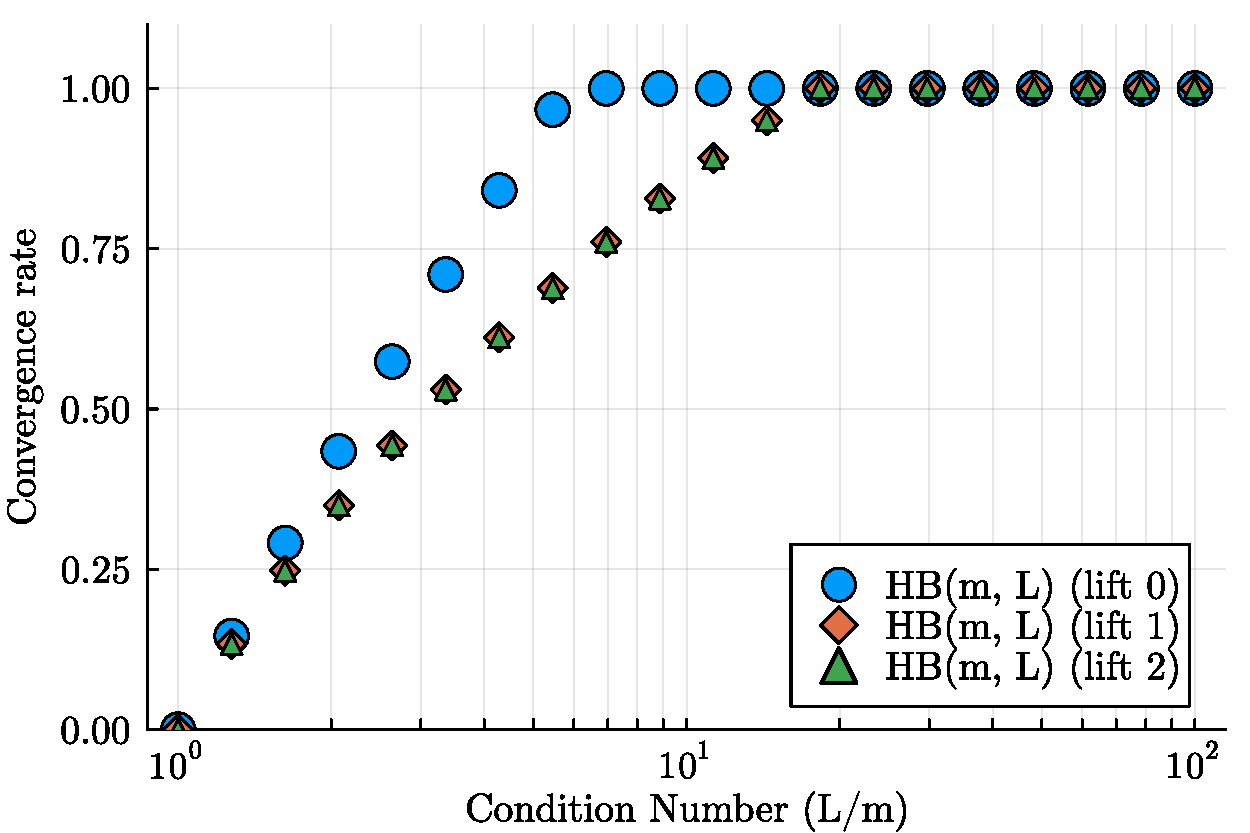
\includegraphics[width = .8 \textwidth]{HBresults.pdf}
    \caption{Convergence rate guarantee of heavy ball with lifting dimensions zero, one, and two, over smooth strongly convex function class}
    \label{HBresults}
\end{figure}

\subsection*{Triple momentum}

We tested the triple momentum algorithm, which was developed by Van Scoy, Freeman, and Lynch in \cite{TMM} to be the fastest known globally convergent first-order algorithm at optimizing strongly convex functions. The algorithm is defined as:
\begin{equation}\label{eqn:TMM}
 x_{k+1}= (1+\beta)x_{k} - \beta x_{k-1} - \alpha \nabla f((1+\gamma)x_k - \gamma x_{k-1})
  \end{equation}

The triple momentum algorithm's optimal parameters are determined by the condition number \( k = L/m \) when optimizing $L$-smooth $m$-strongly convex functions. The algorithm's parameters are defined as:

\[
\begin{aligned}
\rho &= 1 - \frac{1}{\sqrt{k}}, \\
\alpha &= \frac{1 + \rho}{L}, \\
\beta &= \frac{\rho^2}{2 - \rho}, \\
\gamma &= \frac{\rho^2}{(1 + \rho)(2 - \rho)}, \\
% \delta &= \frac{\rho^2}{1 - \rho^2}.
\end{aligned}
\]
Under these parameters, it was proven in \cite{TMM} that the performance guarantee that can be guaranteed the function $1-\sqrt{m/L}$, which is plotted alongside the rates produced by the package in \cref{4_results} as TMM theoretical. The code used to find the worst-case convergence rate guarantees of the triple momentum algorithm is presented in \cref{tmm_code}, with \texttt{m} set to one, \texttt{L} set to the sampled $L$ values, and \texttt{lifting\_dimension} set to one. Note that in \cref{tmm_code}, the performance measure is set to \texttt{((1+delta)*x2 - delta*x1 - xs)\textasciicircum2} in order to get the result in \cref{4_results}. This value is taken from Theorem 1 of \cite{TMM} and adapted to fit the automated analysis in \texttt{AlgorithmAnalysis.jl}, and selecting a different performance measure might not result in analysis figures that match that in Fig.1 of \cite{TMM}.

\begin{figure}[h!]
	\begin{lstlisting}[mathescape]
k = L/m; rho = 1 - 1/(sqrt(k))
$\alpha$ = (1 + rho)/L
$\beta$ = (rho^2)/(2-rho)
gamma = (rho^2)/((1+rho)*(2-rho))
delta = (rho^2)/(1-rho^2)
@algorithm begin
    f = DifferentiableFunctional{R$^n$}()
    xs = first_order_stationary_point(f)
    f $\in$ SmoothStronglyConvex(m, L)
    x0 = R$^n$()
    x1 = R$^n$()
    y1 = (1+gamma)*x1 - gamma*x0
    x2 = (1+$\beta$)*x1 - $\beta$*x0 - $\alpha$*f'(y1)
    x0 => x1
    x1 => x2
    lift(x2, lifting_dimension)
    performance = ((1+delta)*x2 - delta*x1 -xs)^2
end
@show rate(performance)
\end{lstlisting}
\caption{Analysis of triple-momentum and $L$-smooth $m$-strongly convex function class}
\label{tmm_code}
\end{figure}

When we plot the result of analyzing TMM with \texttt{lifting\_dimension} values zero, one, and two, we see the same impact lifting has on the convergence rate guarantee as did FG and HB: not lifting the algorithm produces inaccurate results while creating one or two additional iterates does not affect the result. This can be seen in \cref{TMMresults}.

\begin{figure}[h!]
    \centering
    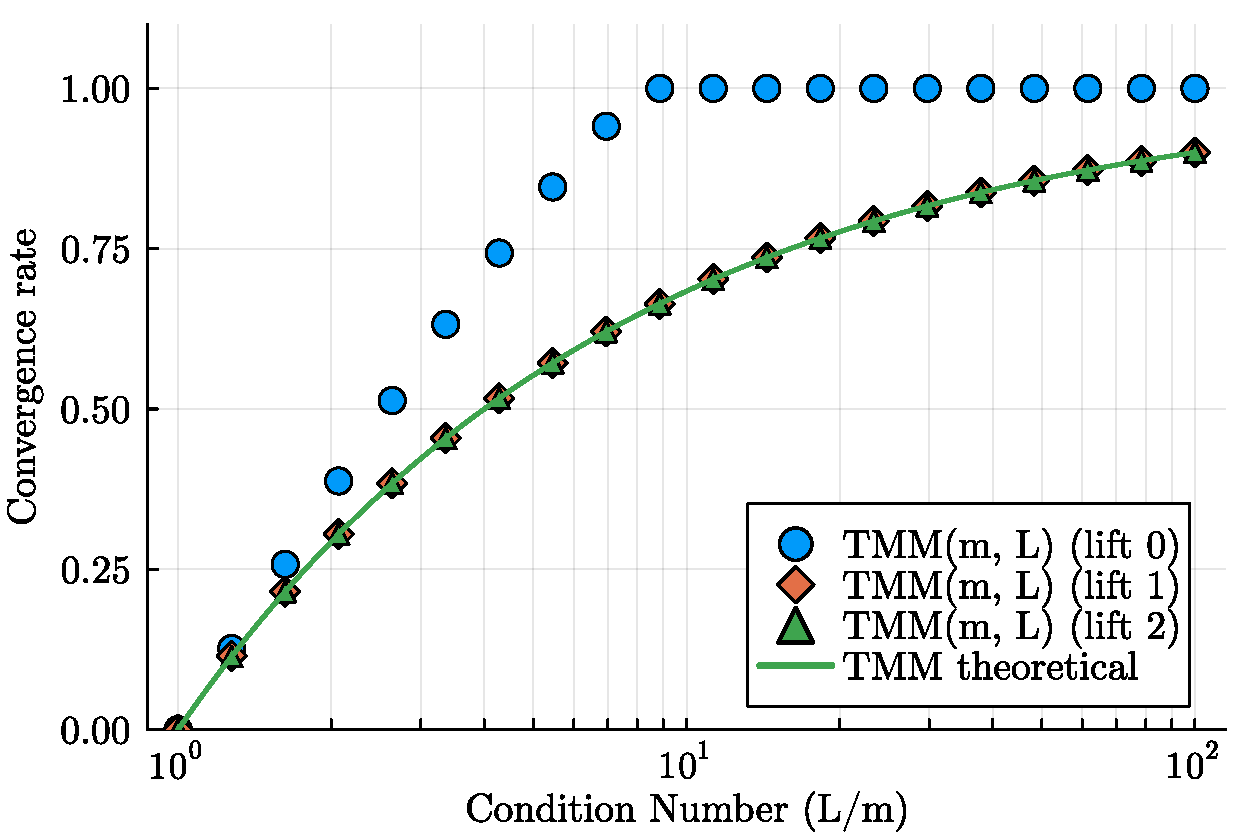
\includegraphics[width = .8 \textwidth]{TMMresults.pdf}
    \caption{Convergence rate guarantee of triple momentum with lifting dimensions zero, one, and two,over smooth strongly convex function classes}
    \label{TMMresults}
\end{figure}